%% Section 6: Results and discussion
\section{Results and Discussion}
\label{sec:results}

\subsection{H4 inverter with unipolar SPWM}
Fig.~\ref{fig:sweepH4U} shows the sweep from 1 to 25~kHz with $L=90$~mH. The leakage current has a sharp peak at 2~kHz, of the order of 0.75~A (the vertical axis of the plot is in amperes; \todo{relabel the axis of the figure as ``A'' or rescale to mA before submission}), accompanied by a dip in efficiency to about 97.0\% and a low-order THD of about 18\%. The peak lies within 3\% of the predicted resonance $\fres=1.94$~kHz. For $\fsw\geq3$~kHz the leakage decays rapidly; at 8.5~kHz it is 15.4~mA with an efficiency of 97.18\% and a THD of 0.16\% (Fig.~\ref{fig:fftH4B} shows a representative FFT for another case). The efficiency is essentially constant (97.2\%) for $\fsw>3$~kHz, which again indicates that switching loss is not modeled in this case. The leakage current falls below 300~mA everywhere except in the neighborhood of the resonance.

\begin{figure*}[!t]
\centering
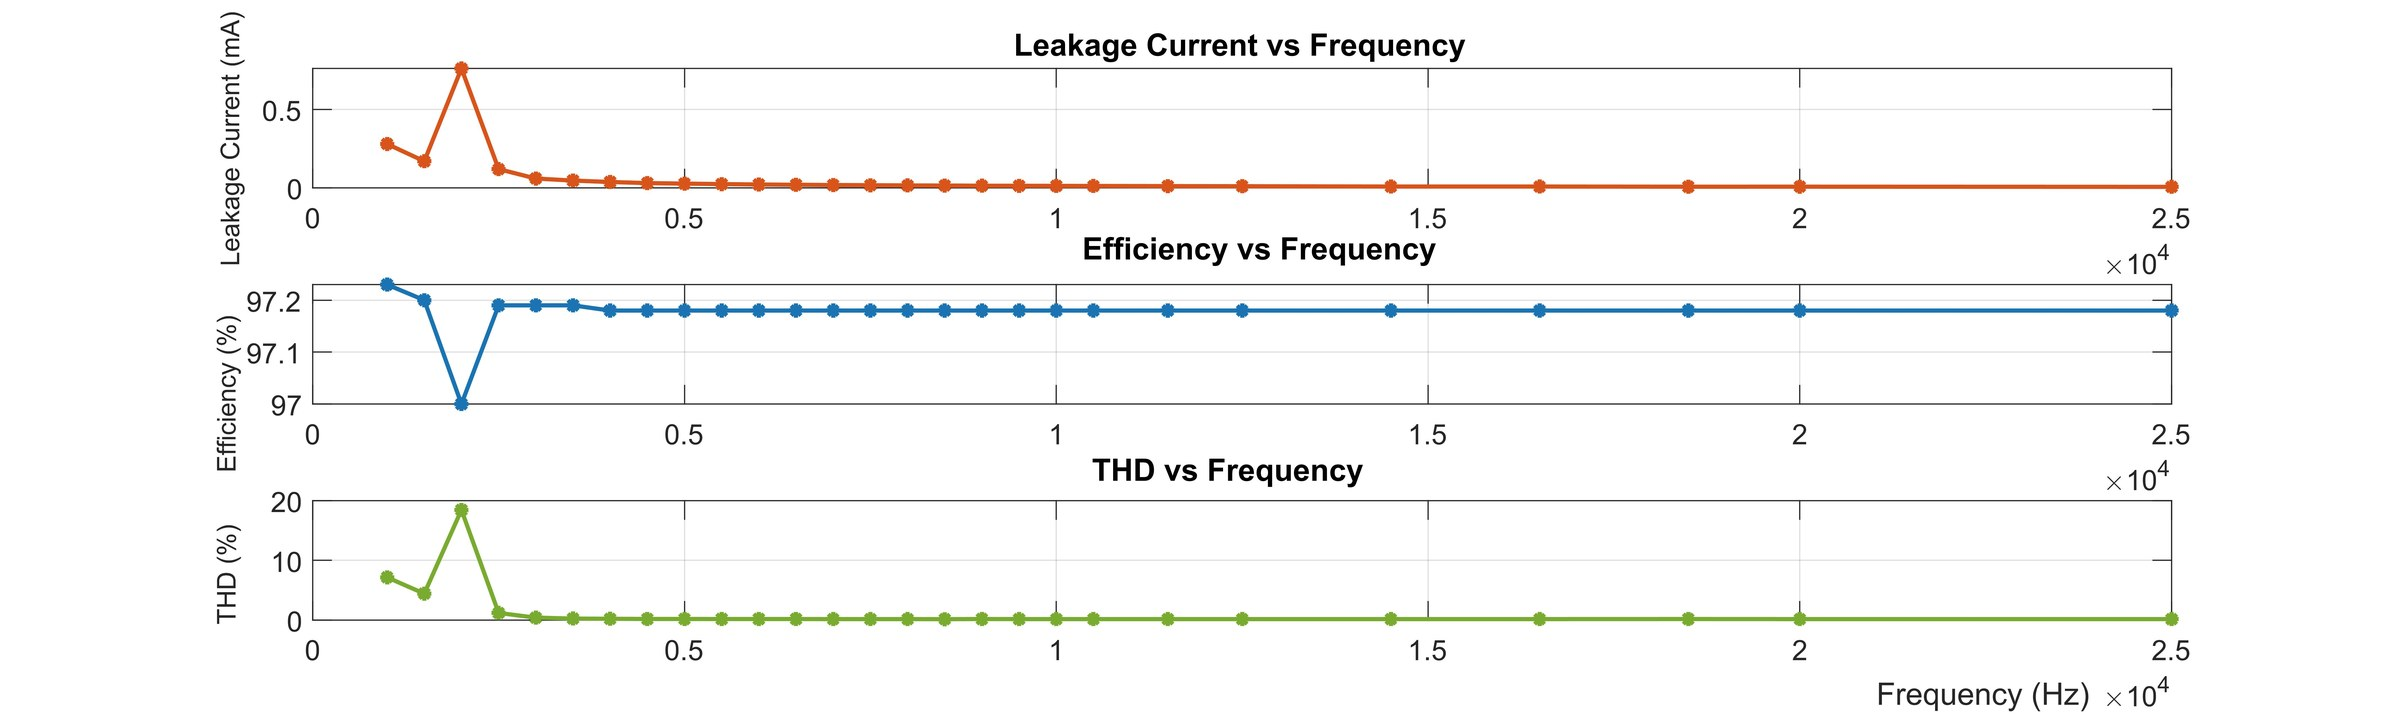
\includegraphics[width=0.85\textwidth]{figures/sweep_h4_unipolar.jpg}
\caption{H4 with unipolar SPWM: leakage current, efficiency and low-order THD versus switching frequency ($\Vdc=220$~V, $L_1=L_2=90$~mH, $R_L=50\;\Omega$, $\Cpv=150$~nF). \todo{The leakage axis is labelled mA in the source plot but its values correspond to amperes; correct before submission.}}
\label{fig:sweepH4U}
\end{figure*}

The CMV and leakage waveforms at the start of the simulation (Fig.~\ref{fig:wavesH4U}) confirm the mechanism. The CMV is a rectified-sine-like envelope carrying a carrier-frequency ripple, characteristic of unipolar modulation, and the leakage current exhibits a decaying start-up oscillation superimposed on a steady-state ripple that is amplitude-modulated at twice the line frequency.

\begin{figure}[!t]
\centering
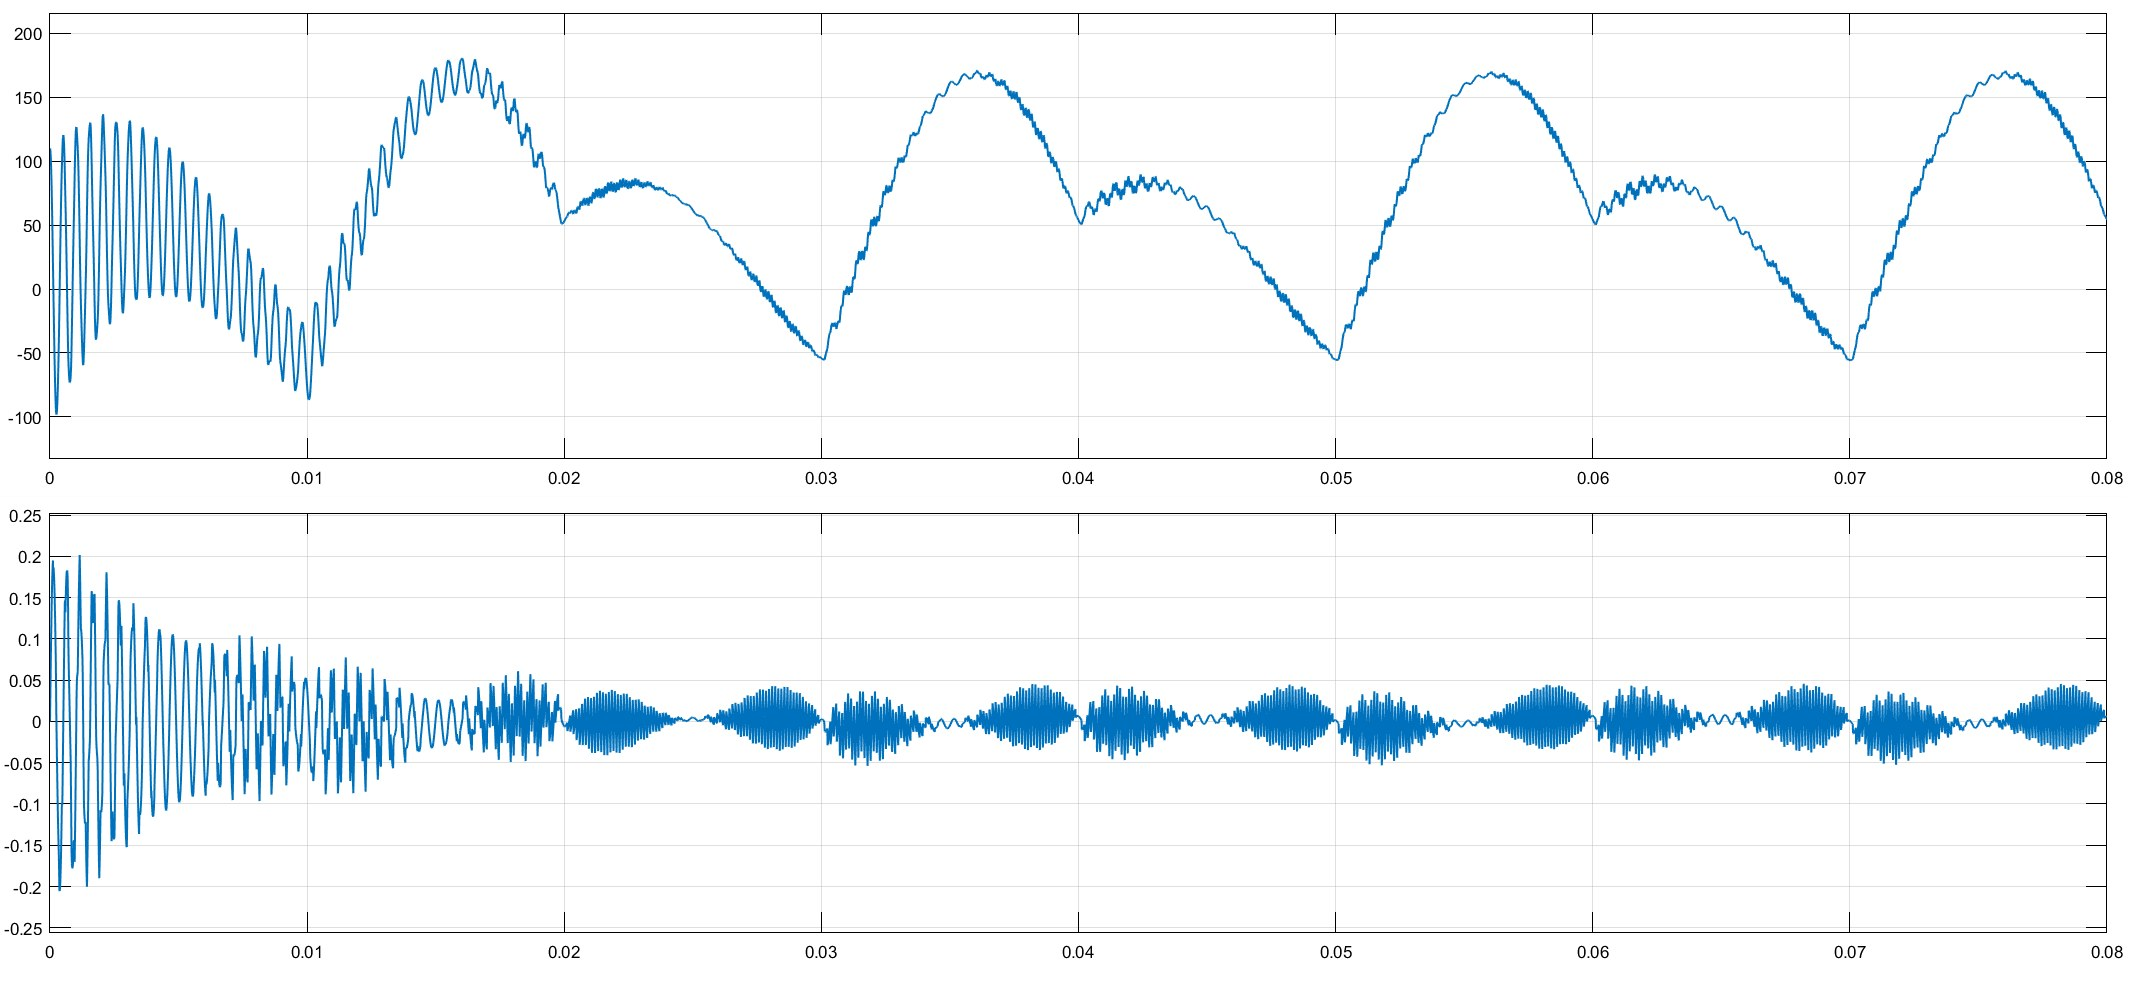
\includegraphics[width=\columnwidth]{figures/wave_h4_unipolar_cmv.jpg}
\caption{H4 with unipolar SPWM: (top) CMV in volts and (bottom) leakage current in amperes. The start-up transient decays within about two line cycles.}
\label{fig:wavesH4U}
\end{figure}

\subsection{H4 inverter with bipolar SPWM}
Fig.~\ref{fig:sweepH4B} shows the sweep from 1 to 40~kHz with $\Vdc=460$~V and $L=10$~mH. The leakage current is non-monotonic: there are strong peaks of about 500~mA at 2~kHz and about 440~mA at 12~kHz, a smaller peak of about 160~mA at 5~kHz, and a broad hump of about 120~mA near 25~kHz. For $\fsw\geq13$~kHz the leakage is in the range 20--60~mA up to 20~kHz and decreases to 14~mA at 40~kHz. The efficiency decreases from about 98.2\% at 1--2~kHz to 97.7\% at 15--40~kHz, with dips to 96.9\% at 6 and 10~kHz. The low-order THD is 33\% at 1~kHz, which is consistent with the large ripple at that frequency ($\Delta I_{pp,\max}\approx11.5$~A for $\Vdc=460$~V, $L=10$~mH, $\fsw=1$~kHz relative to a load-current amplitude of about 38~A), and falls below 0.2\% for $\fsw\geq5$~kHz. At 40~kHz the leakage current is 14~mA, the efficiency 97.72\% and the THD 0.10\% (Fig.~\ref{fig:fftH4B}).

The voltage across $\Cpv$ in this case (Fig.~\ref{fig:wavesH4B}) is a 50-Hz sinusoid between about 40 and 420~V, i.e., of amplitude about 190~V about a mean of $\Vdc/2=230$~V. This is half of the 384-V output amplitude and agrees with the effective source \eqref{eq:tcm}: even though the CMV of the bipolar bridge is constant on average, the grounded load terminal adds a term $-v_o/2$. Equation~\eqref{eq:floor} gives a line-frequency floor of 6.4~mA for this amplitude, below the 14~mA measured at 40~kHz.

\begin{figure}[!t]
\centering
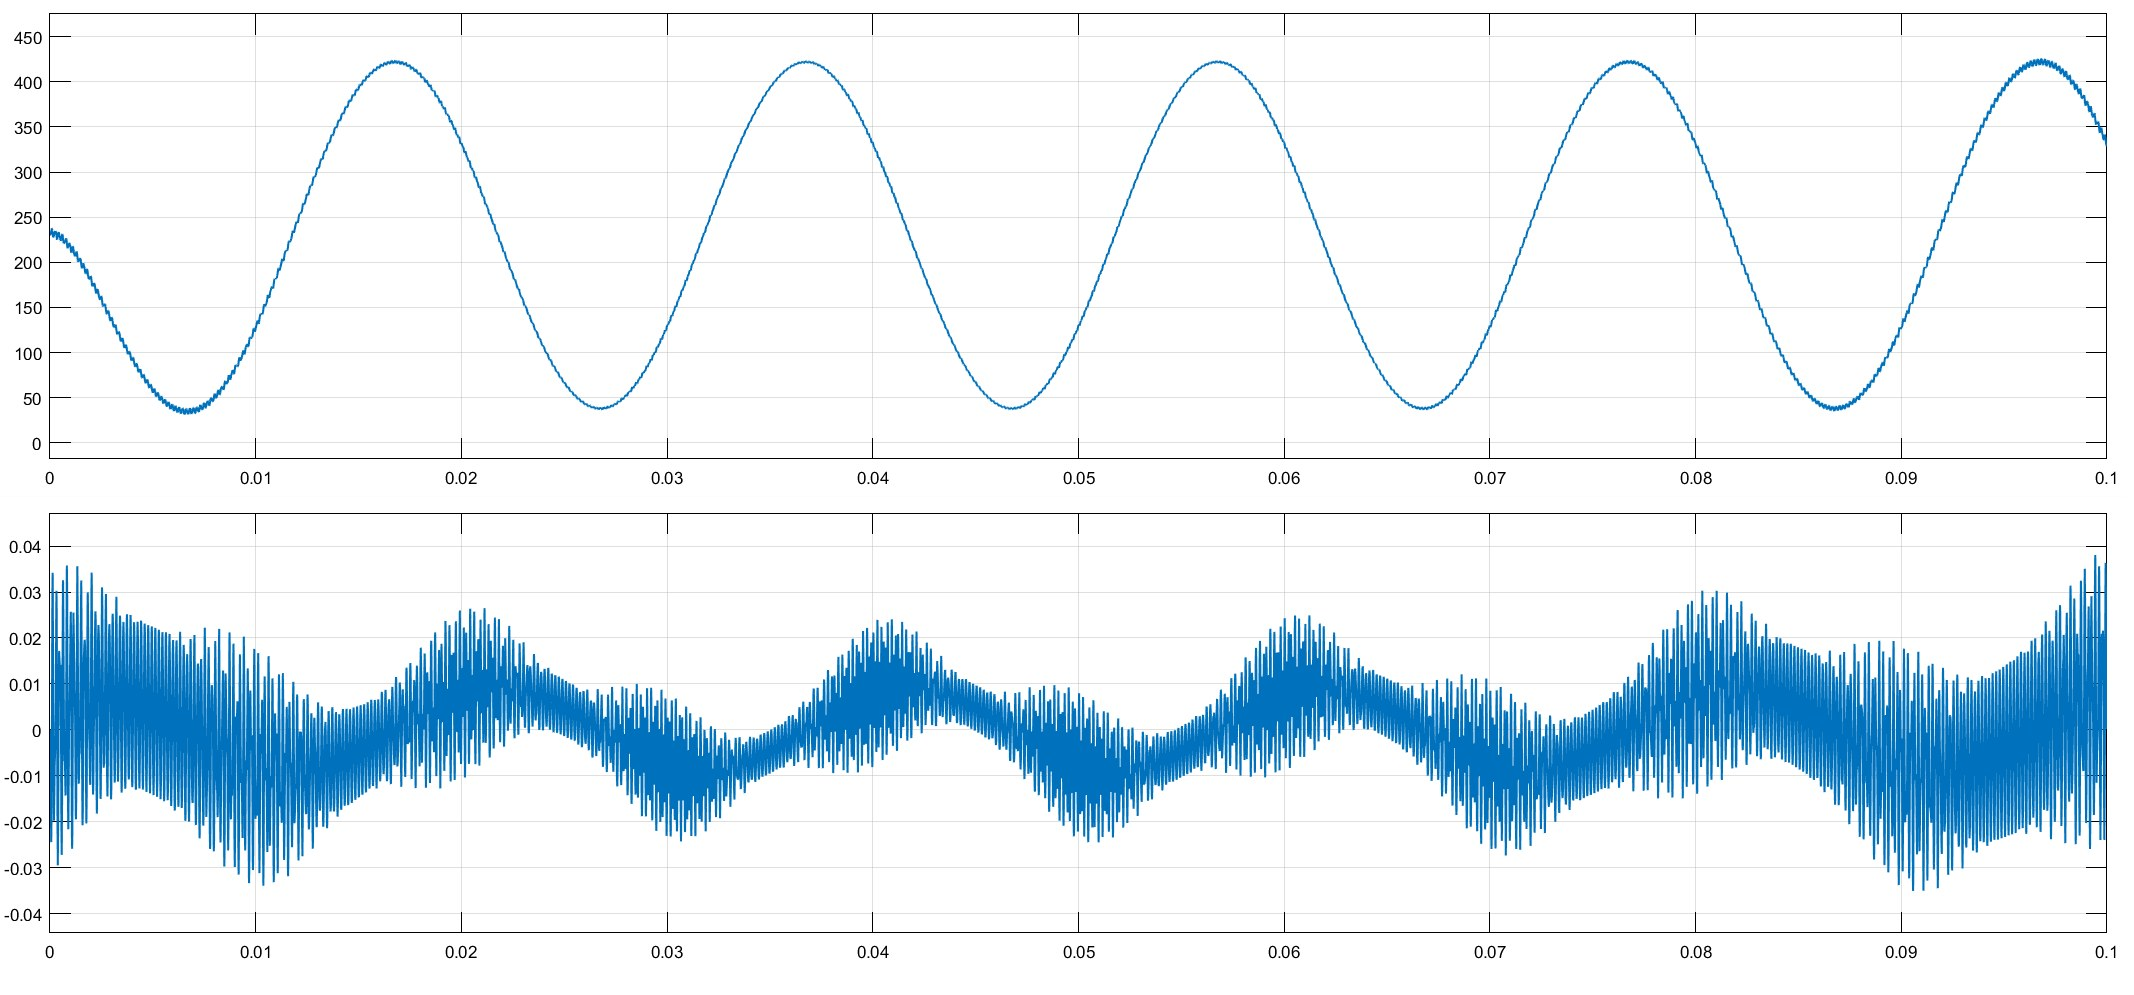
\includegraphics[width=\columnwidth]{figures/wave_h4_bipolar_cmv.jpg}
\caption{H4 with bipolar SPWM at the start of the simulation: (top) voltage across $\Cpv$ in volts and (bottom) leakage current in amperes.}
\label{fig:wavesH4B}
\end{figure}

Both major peaks fall at predicted frequencies, but by different mechanisms. The 2-kHz peak lies at $\fres/3=1.94$~kHz, so that $3\fsw\approx\fres$, as expected from the third harmonic of the carrier exciting the resonance. The 12-kHz peak lies at $2\fres=11.6$~kHz, which the mechanism of Section~\ref{sec:cm} does not predict, because it would require sub-harmonic content at $\fsw/2$ in the effective source. The smaller 5-kHz hump lies 14\% below $\fres$, which exceeds the 1-kHz sweep step; it is treated as a secondary feature that the first-order model does not explain (for example, a damping-related shift or an interaction with the DC-link and source impedance).

\begin{figure*}[!t]
\centering
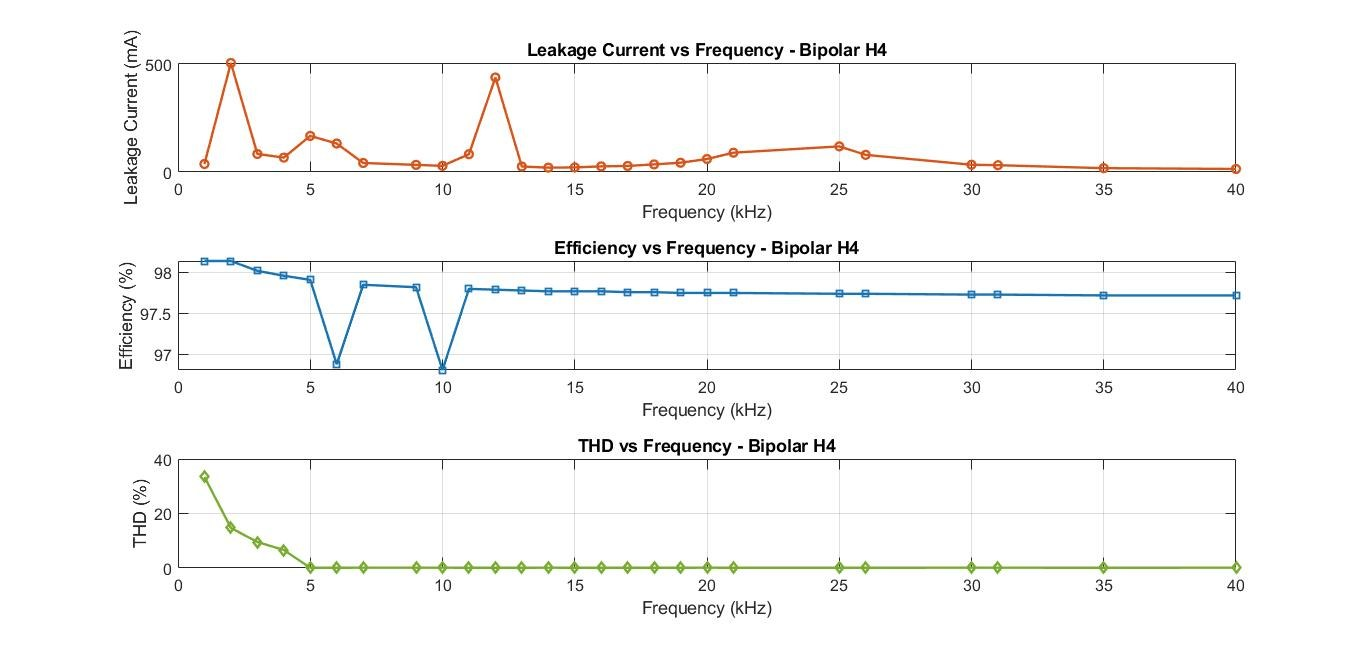
\includegraphics[width=0.85\textwidth]{figures/sweep_h4_bipolar.jpg}
\caption{H4 with bipolar SPWM: leakage current (mA), efficiency and THD versus switching frequency ($\Vdc=460$~V, $L_1=L_2=10$~mH, $R_L=10\;\Omega$, $\Cpv=150$~nF).}
\label{fig:sweepH4B}
\end{figure*}

\begin{figure}[!t]
\centering
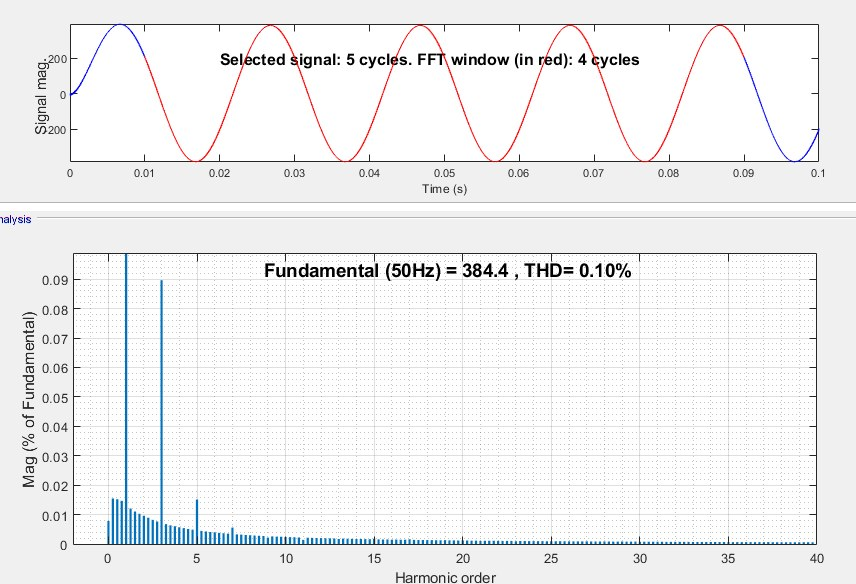
\includegraphics[width=\columnwidth]{figures/fft_h4_bipolar.jpg}
\caption{Powergui FFT of the H4 bipolar output voltage at 40~kHz: fundamental 384.4~V, THD $=0.10\%$ (harmonic orders up to 40; 5 simulated cycles, 4-cycle window).}
\label{fig:fftH4B}
\end{figure}

\subsection{Effect of the L filter on the output waveform}
Fig.~\ref{fig:h4out} shows the H4 unipolar output voltage before and after the filter. The unfiltered voltage is a three-level PWM waveform of $\pm220$~V; the filter removes the switching ripple and leaves a sinusoid with a start-up transient. The Powergui FFT, restricted to harmonic orders up to 40, gives a THD of 0.28\% before and 0.16\% after the filter. These numbers are small for both waveforms because the band covers only up to 2~kHz and therefore excludes the switching sidebands, which are the actual difference between the two waveforms. The low-order THD is thus a measure of the fundamental-band distortion (dead time, crossover, start-up transient), and the ripple attenuation of the filter is better evaluated from the waveform (Fig.~\ref{fig:h4out}) or from a wide-band FFT. A wide-band FFT, together with the compliance with the harmonic limits of \cite{IEEE519,IEEE1547} that depend on the short-circuit ratio of the point of connection, is part of the future work.

\begin{figure}[!t]
\centering
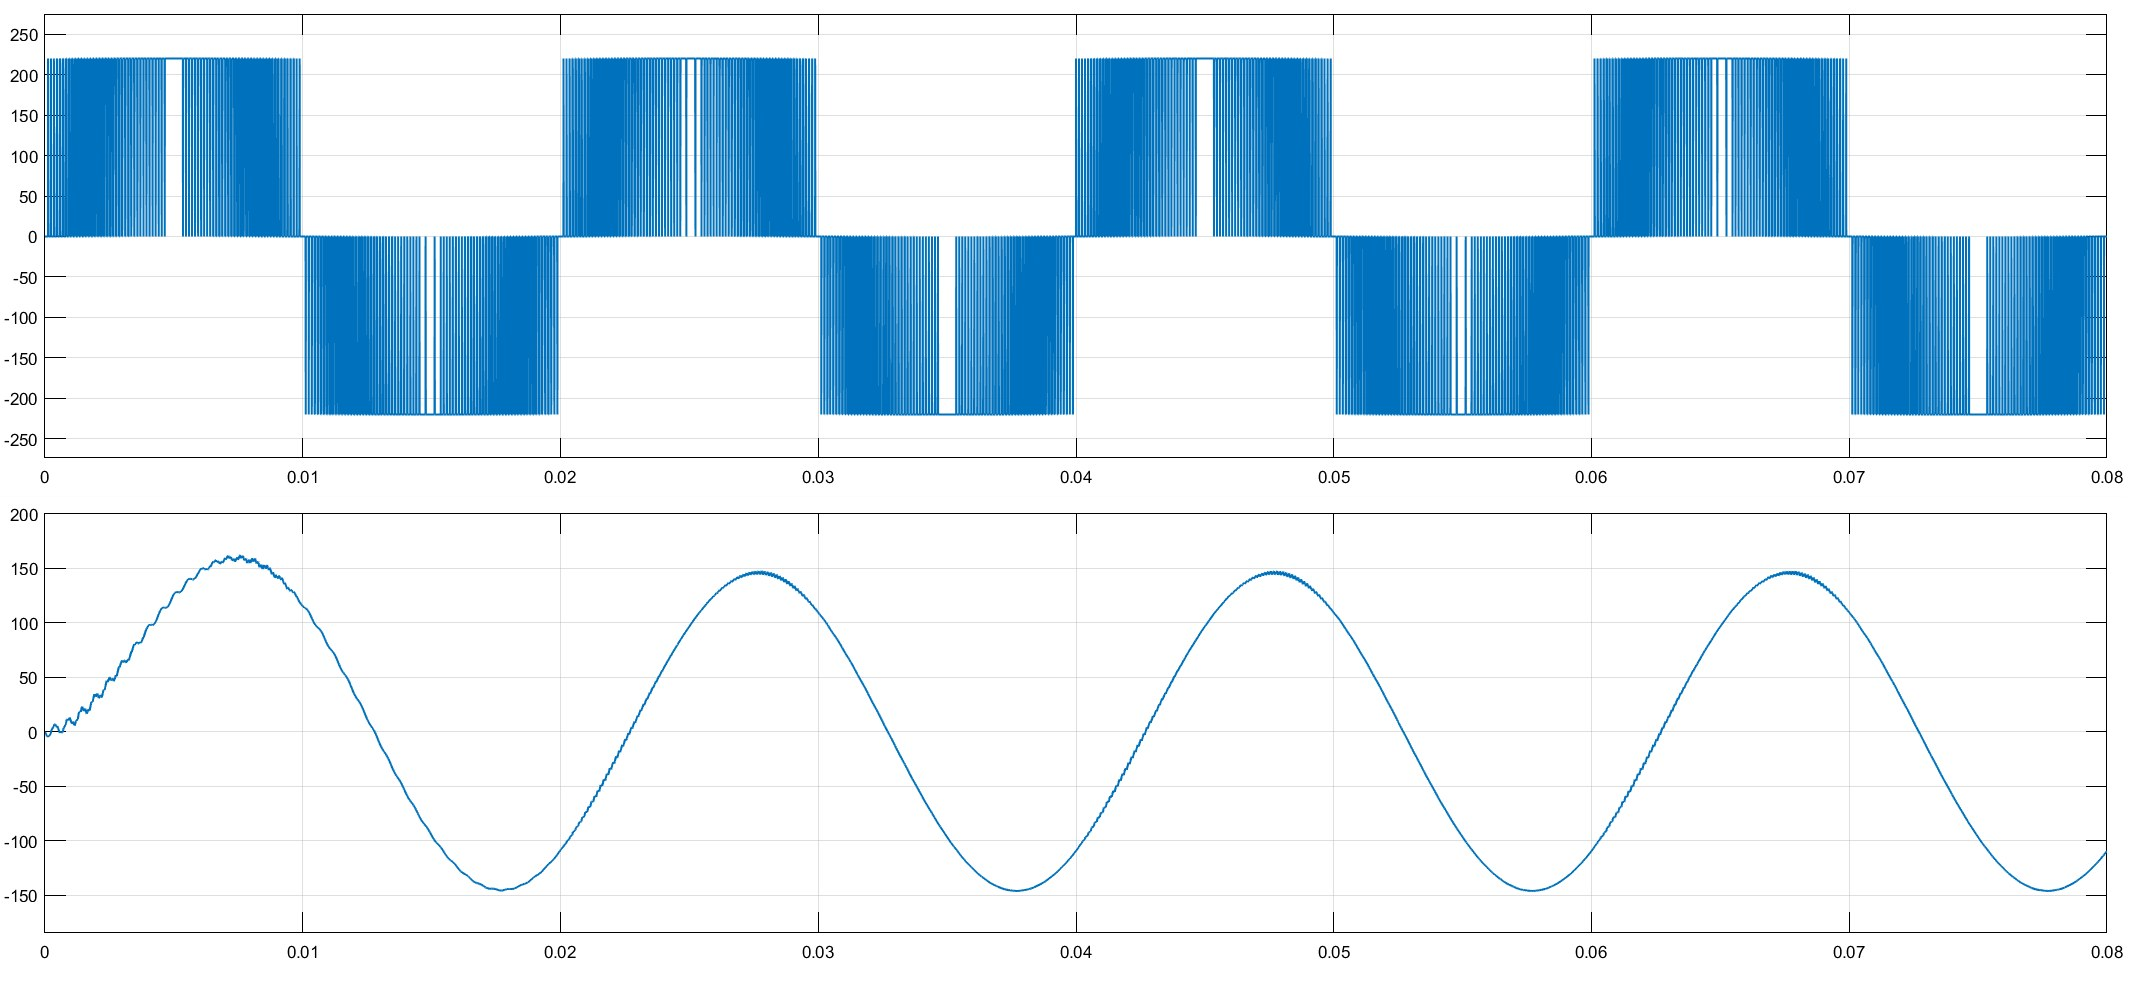
\includegraphics[width=\columnwidth]{figures/wave_h4_unipolar_out.jpg}
\caption{H4 with unipolar SPWM: (top) unfiltered and (bottom) filtered output voltage in volts ($\Vdc=220$~V, $L_1=L_2=90$~mH).}
\label{fig:h4out}
\end{figure}

\subsection{HERIC inverter with unipolar SPWM}
For HERIC with unipolar SPWM ($\Vdc=220$~V, $L=10$~mH, $R_L=10.68\;\Omega$) the sweep of 5--30~kHz in Fig.~\ref{fig:sweepHU} shows the most pronounced resonance of all cases: the leakage current rises from about 0.6~A at 5~kHz to a maximum of about 4~A at 6~kHz and falls steeply, to about 0.5~A at 7~kHz, and then more slowly to a few tens of milliamps above 20~kHz. The peak is within 3\% of the predicted $\fres=5.81$~kHz. At 26~kHz the leakage is 40.27~mA, the efficiency is 98.97\% and the low-order THD is 0.05\%. The efficiency is virtually independent of $\fsw$ (98.93--98.97\%, with a minimum at the resonance), and the THD increases only slightly from 0.05\% (up to about 16~kHz) to 0.09\% near 30~kHz. Fig.~\ref{fig:fftHU} shows the corresponding FFT. In this model the CMV is not constant: the CM and leakage waveforms (Fig.~\ref{fig:wavesHU}) display a 100-Hz rectified-sine envelope with high-frequency ripple, i.e., the AC bypass does not fully decouple the PV array during the zero-voltage interval; this is consistent with the leakage current of tens of mA at 26~kHz, an order of magnitude above the HERIC bipolar case. Keeping the leakage below 300~mA requires, from the plot, $\fsw\gtrsim9$~kHz.

\begin{figure}[!t]
\centering
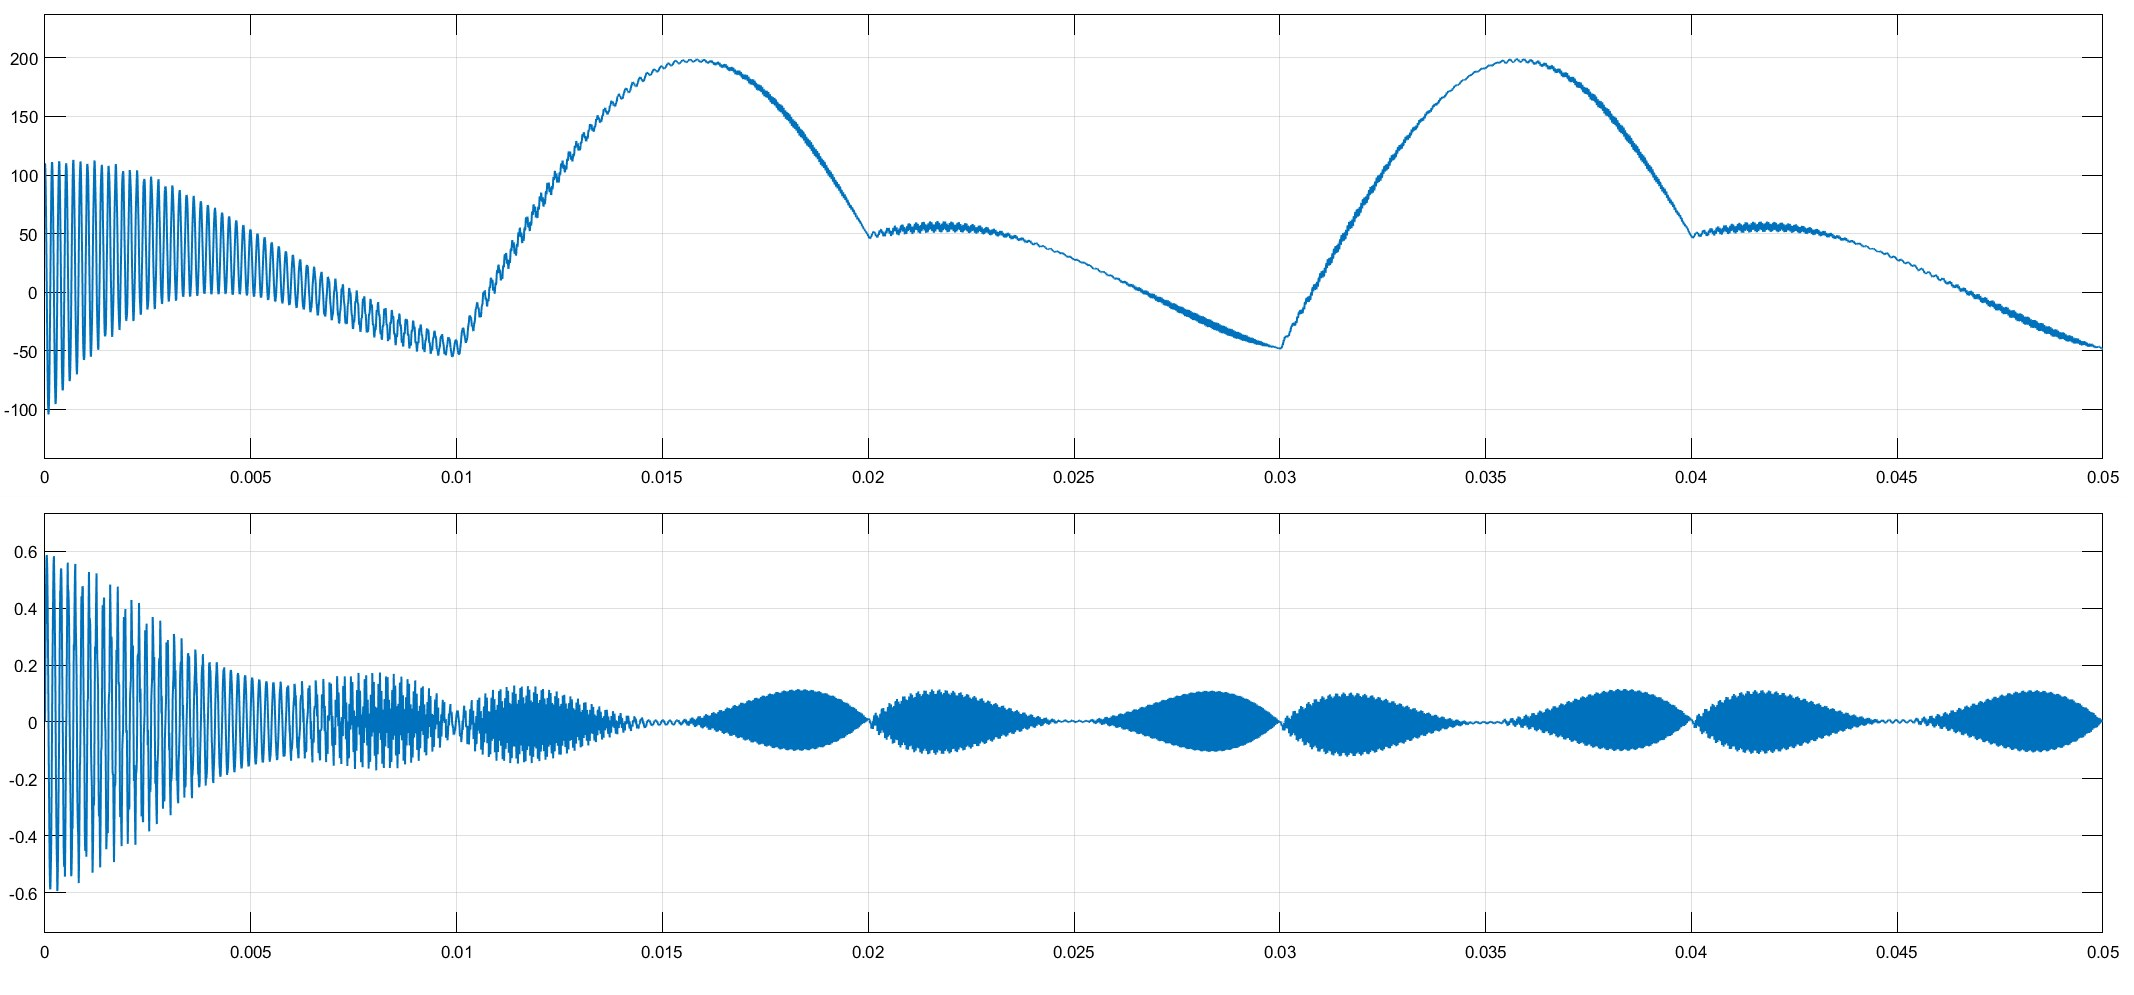
\includegraphics[width=\columnwidth]{figures/wave_heric_unipolar_cmv.jpg}
\caption{HERIC with unipolar SPWM: (top) voltage across $\Cpv$ in volts and (bottom) leakage current in amperes. The envelope repeats at 100~Hz, so the decoupling by the bypass is incomplete in the model.}
\label{fig:wavesHU}
\end{figure}

\begin{figure*}[!t]
\centering
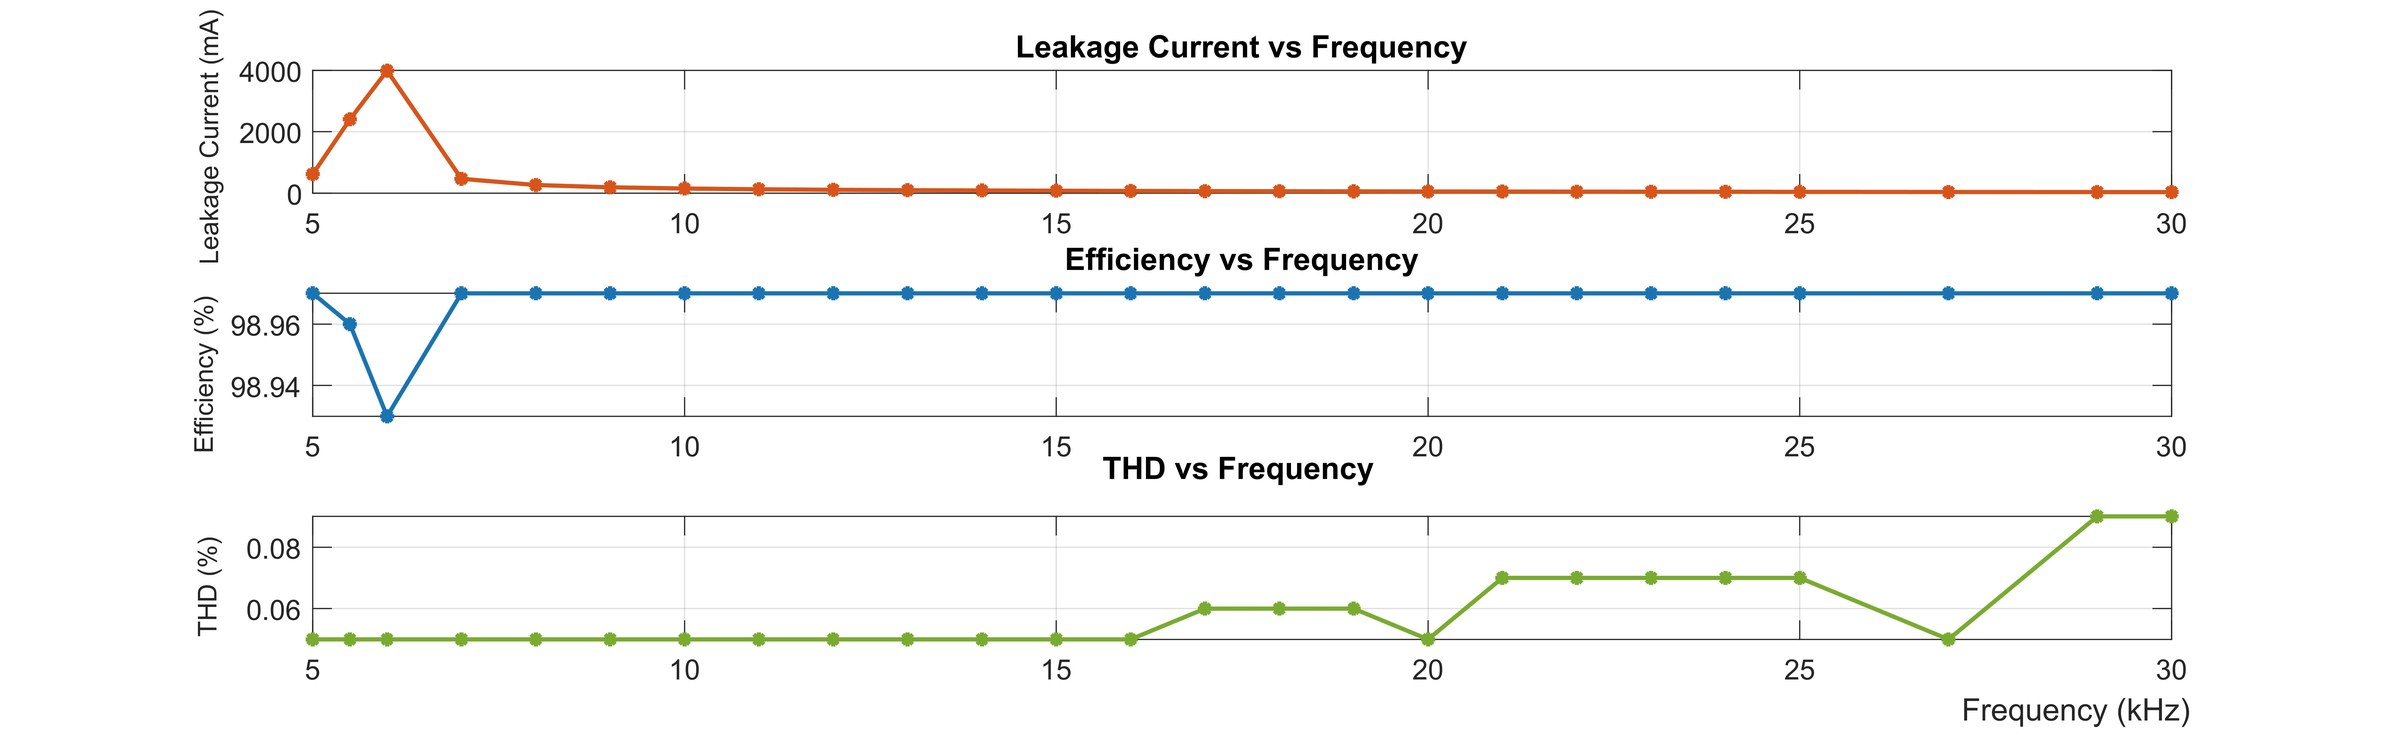
\includegraphics[width=0.85\textwidth]{figures/sweep_heric_unipolar.jpg}
\caption{HERIC with unipolar SPWM: leakage current (mA), efficiency and low-order THD versus switching frequency ($\Vdc=220$~V, $L_1=L_2=10$~mH, $R_L=10.68\;\Omega$, $\Cpv=150$~nF).}
\label{fig:sweepHU}
\end{figure*}

\begin{figure}[!t]
\centering
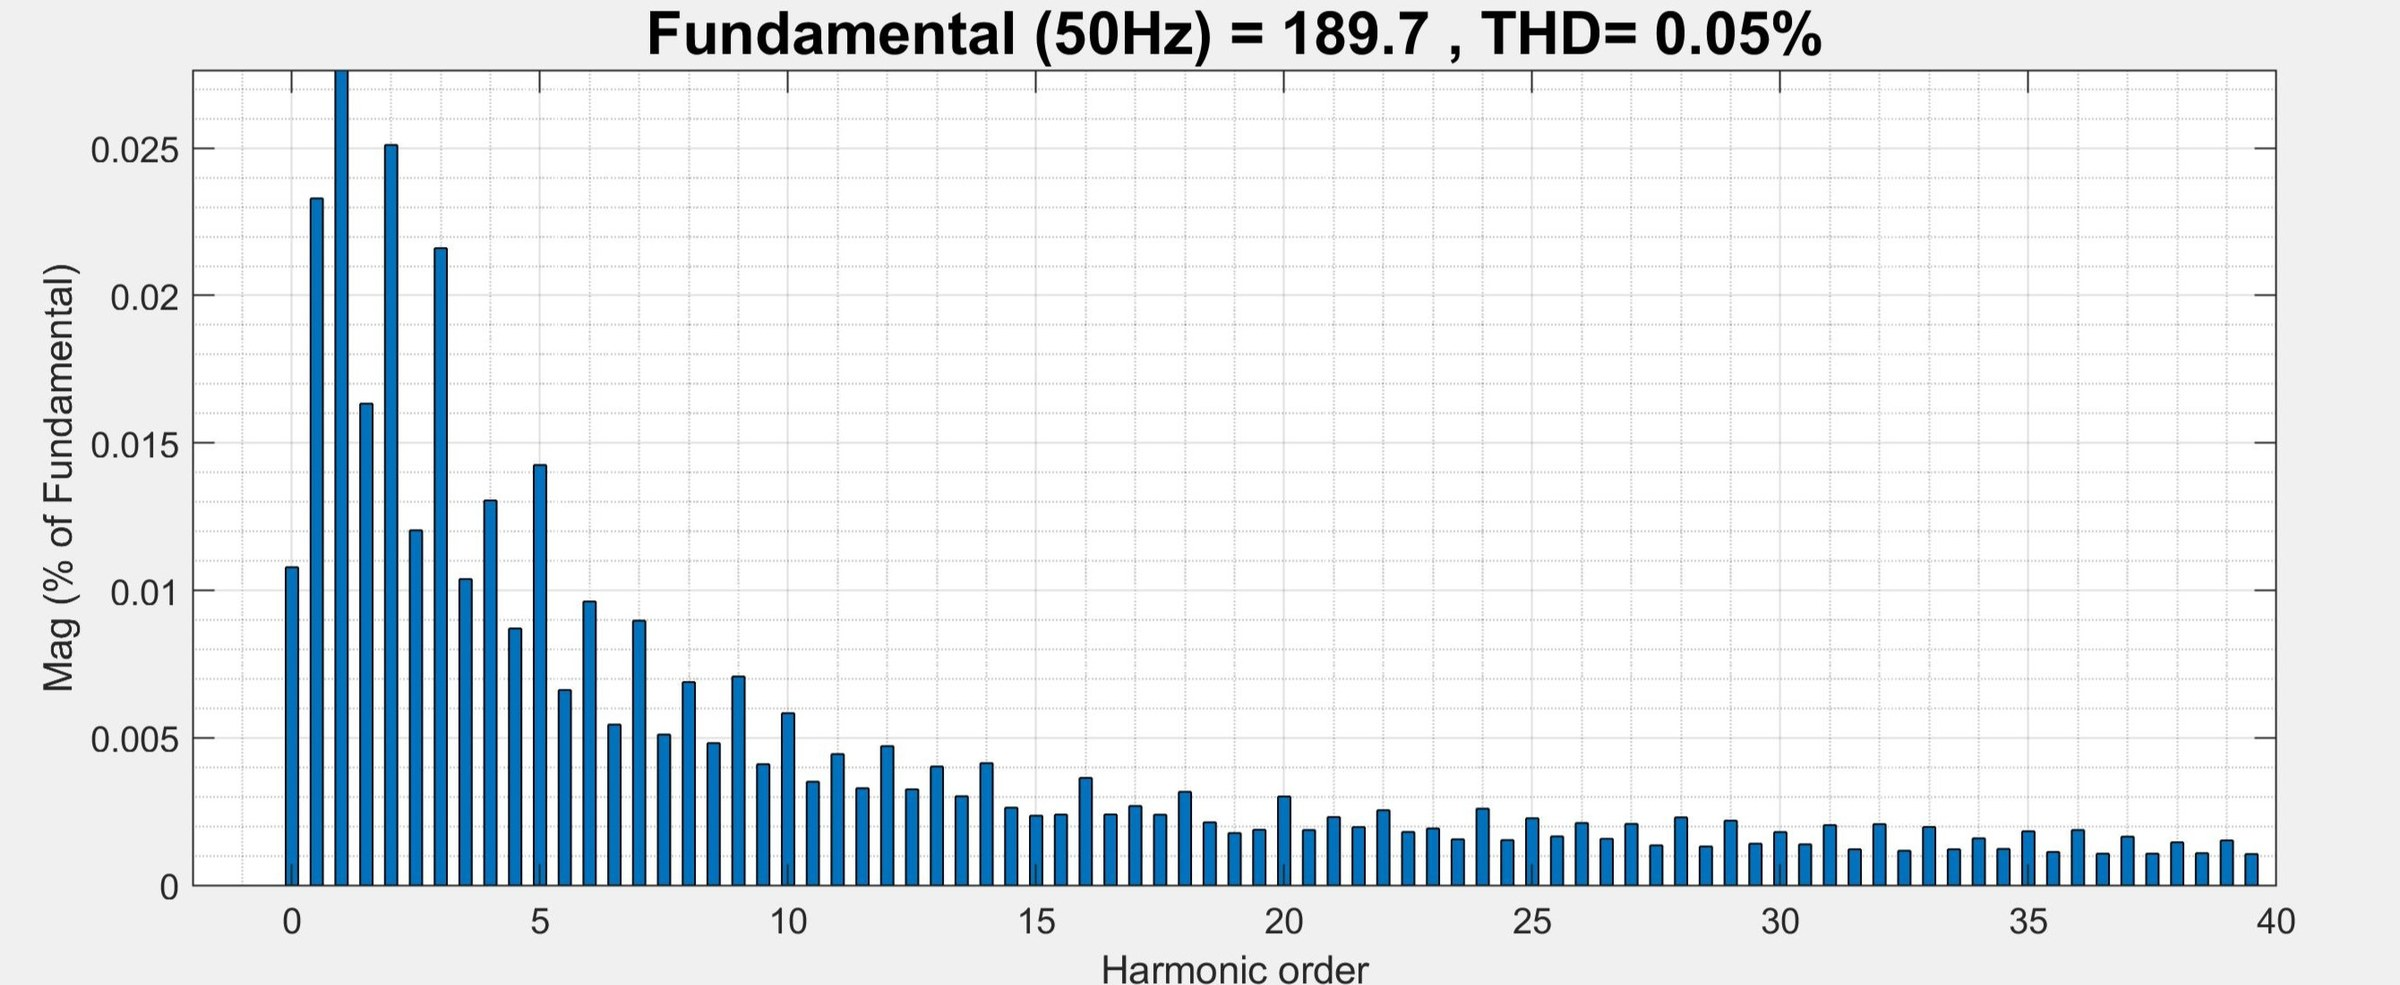
\includegraphics[width=\columnwidth]{figures/fft_heric_unipolar.jpg}
\caption{Powergui FFT of the HERIC unipolar output voltage with the filter: fundamental 189.7~V, THD $=0.05\%$ (harmonic orders up to 40).}
\label{fig:fftHU}
\end{figure}

\subsection{HERIC inverter with bipolar SPWM}
With bipolar SPWM and identical circuit parameters, the HERIC leakage current is much lower (Fig.~\ref{fig:sweepHB}): it has a modest maximum of about 15~mA at 5.5~kHz, which lies 5\% below the predicted $\fres$, falls to a minimum of about 3.2~mA at 10--10.5~kHz, and then rises slowly to about 5.5~mA at 35~kHz. At 13.5~kHz the leakage is 3.53~mA, and the low-order THD is 9.11\%. The leakage at the resonance is only about four times the floor, because the HF CMV content is small and the resonance has little to excite.

\begin{figure*}[!t]
\centering
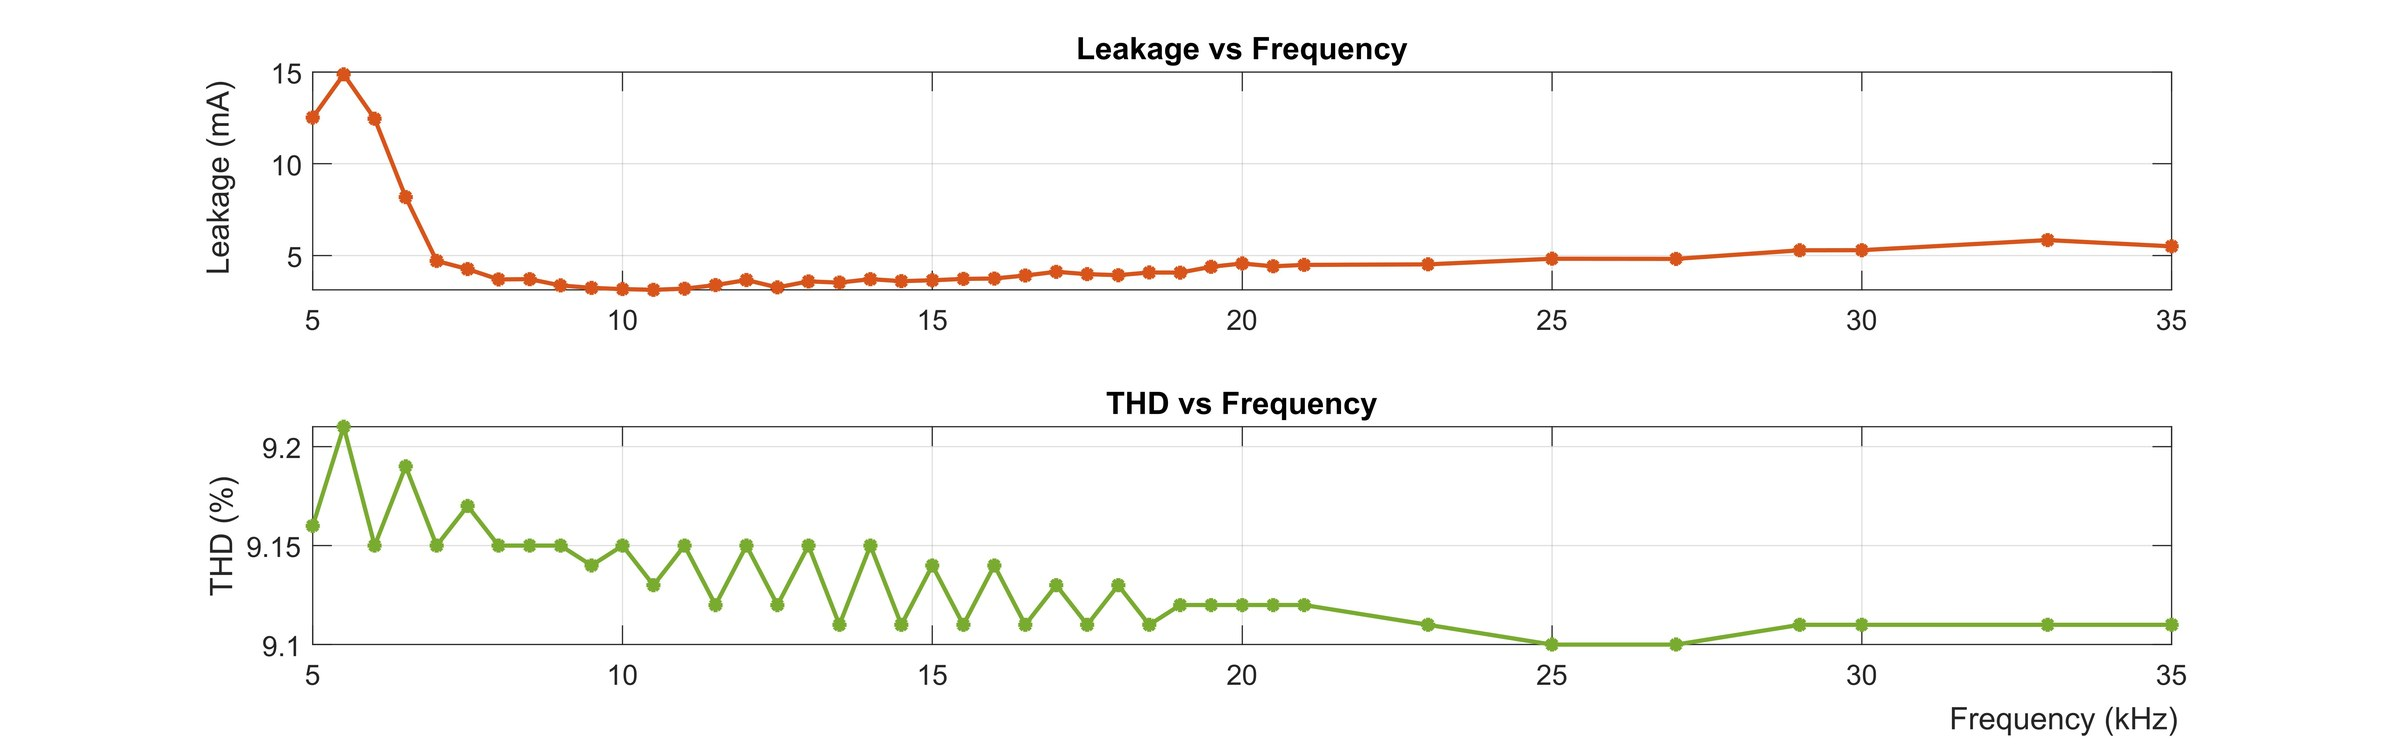
\includegraphics[width=0.85\textwidth]{figures/sweep_heric_bipolar.jpg}
\caption{HERIC with bipolar SPWM: leakage current (mA) and low-order THD versus switching frequency ($\Vdc=220$~V, $L_1=L_2=10$~mH, $R_L=10.68\;\Omega$, $\Cpv=150$~nF). An efficiency sweep was not recorded for this case.}
\label{fig:sweepHB}
\end{figure*}

\emph{Origin of the leakage floor.} The voltage across $\Cpv$ in this case (Fig.~\ref{fig:wavesHB}) is a smooth line-frequency waveform swinging between about 15 and 205~V, i.e., a 50-Hz component of about 95~V peak, which is half of the 190-V output amplitude, as \eqref{eq:tcm} predicts. Using~\eqref{eq:floor} with $V_{o,pk}=190$~V and $\Cpv=150$~nF gives $I_{\mathrm{floor}}\approx3.2$~mA, which matches the measured minimum of 3.2--3.5~mA. The leakage floor of this configuration is therefore the displacement current of the 50-Hz term of \eqref{eq:tcm} in $\Cpv$, not a switching-frequency effect, which explains why it is almost independent of $\fsw$ away from the resonance and implies that the bipolar HERIC configuration has essentially no carrier-frequency CMV in the simulation. (The 190-V amplitude is read from Fig.~\ref{fig:wavesHB}; the agreement should be regarded as an order-of-magnitude consistency check.) Table~\ref{tab:floor} applies the same estimate to the other cases: the line-frequency floor is 3--6~mA, so the leakage of 14--40~mA reported for the other three operating points is dominated by carrier-frequency components of $\vCM$. For H4 unipolar this is by design; for HERIC unipolar the bypass does not fully decouple the PV array in the model; for H4 bipolar the excess over the floor (about 8~mA at 40~kHz, and the large resonant peaks elsewhere) indicates a residual carrier-frequency CMV whose origin (switch parasitics, DC-source impedance or ripple asymmetry) was not isolated in this study.

\begin{table}[!t]
\renewcommand{\arraystretch}{1.2}
\caption{Line-frequency leakage floor from \eqref{eq:floor} versus reported operating points ($\Cpv=150$~nF)}
\label{tab:floor}
\centering
\footnotesize
\begin{adjustbox}{max width=\columnwidth}
\begin{tabular}{lcccc}
\toprule
Case & $V_{o,pk}$ (V) & $I_{\mathrm{floor}}$ (mA) & Operating point (kHz) & $I_{\mathrm{leak}}$ (mA) \\
\midrule
H4, unipolar & 220 & 3.7 & 8.5 & 15.4 \\
H4, bipolar & 384 & 6.4 & 40 & 14 \\
HERIC, unipolar & 190 & 3.2 & 26 & 40.3 \\
HERIC, bipolar & 190 & 3.2 & 13.5 & 3.5 \\
\bottomrule
\end{tabular}
\end{adjustbox}
\end{table}

\begin{figure}[!t]
\centering
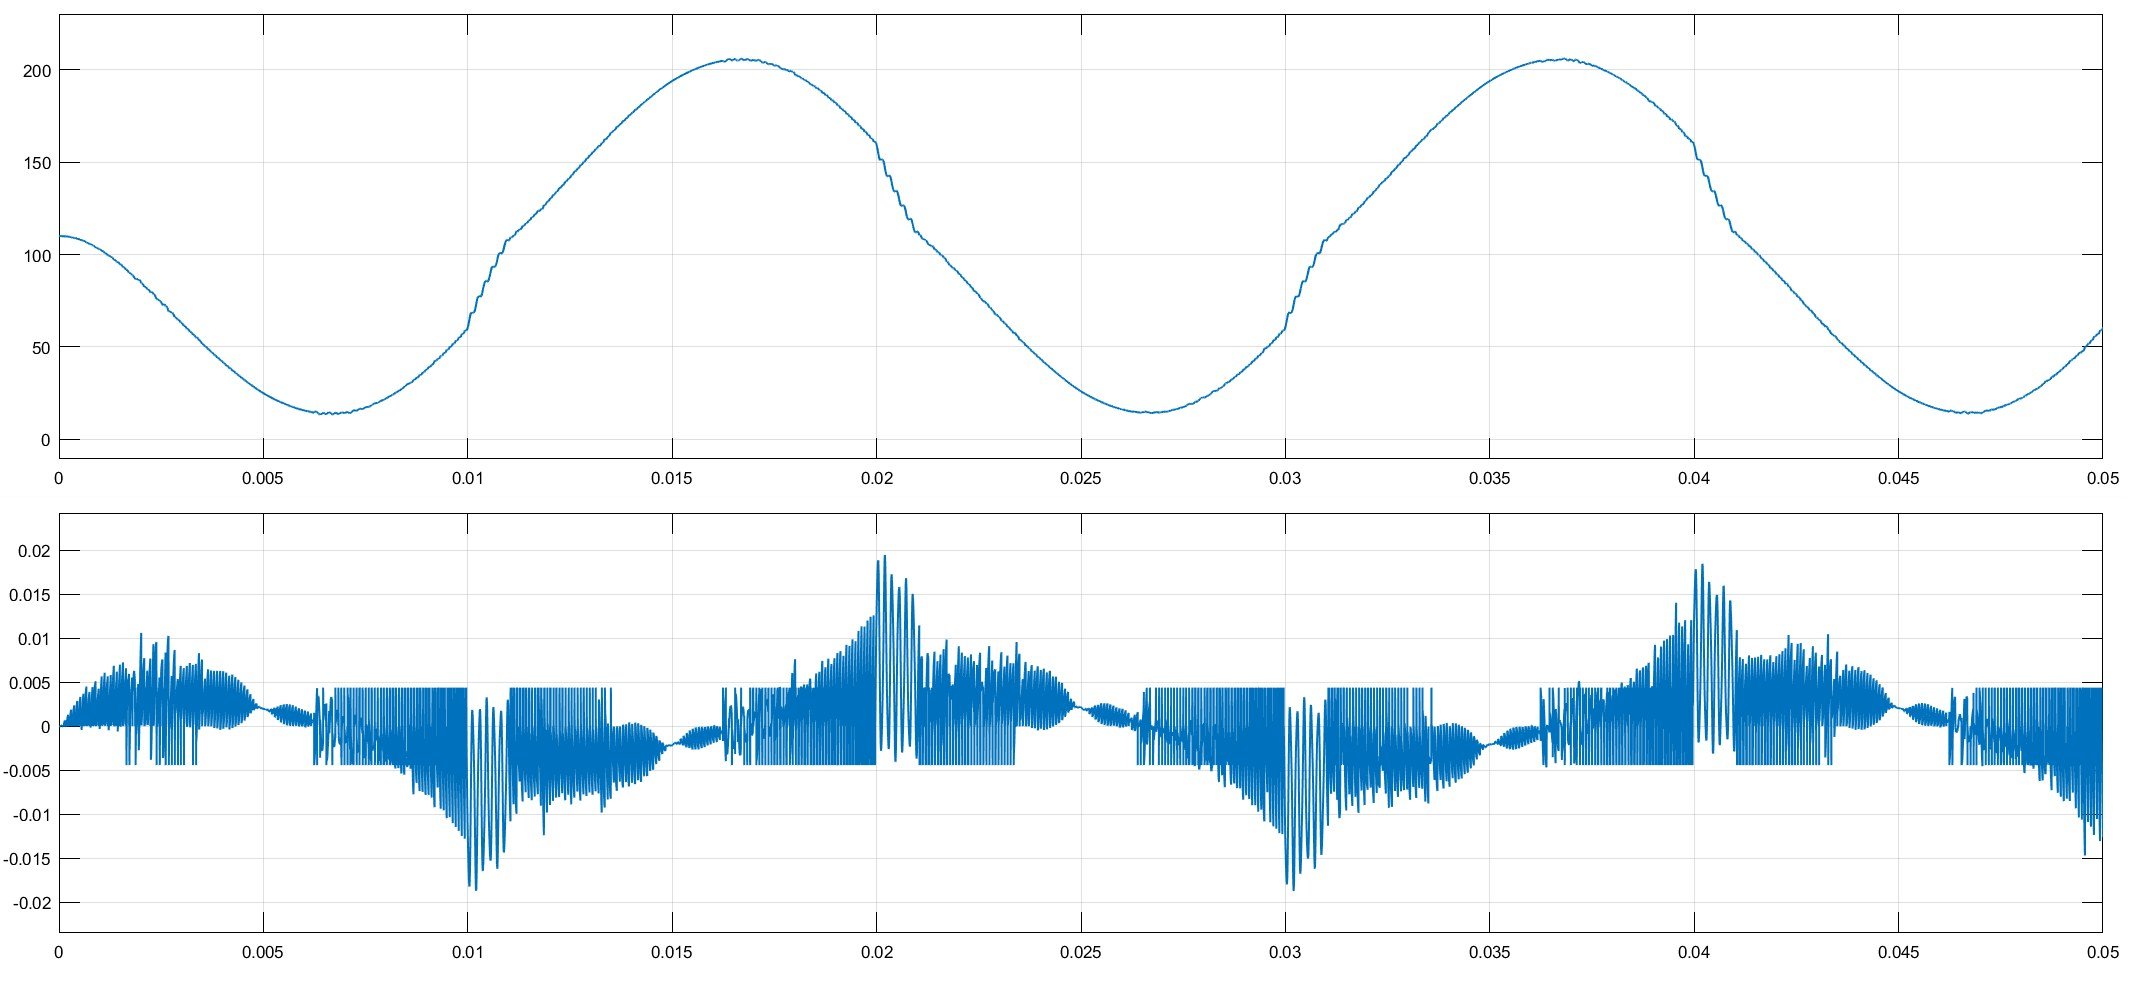
\includegraphics[width=\columnwidth]{figures/wave_heric_bipolar_cmv.jpg}
\caption{HERIC with bipolar SPWM: (top) CMV in volts and (bottom) leakage current in amperes.}
\label{fig:wavesHB}
\end{figure}

\emph{Origin of the THD.} The low-order THD of 9.1--9.2\% is almost constant over the entire sweep (5--35~kHz, Fig.~\ref{fig:sweepHB}). If it were caused by insufficient filtering of the switching ripple, it would decrease as $\fsw$ increases. Its invariance indicates a low-frequency origin. The filtered output voltage (Fig.~\ref{fig:outHB}) shows kinks at the zero crossings, i.e., crossover distortion, which is consistent with the interaction between the bipolar bridge modulation and the line-frequency bypass gating, and with the large DC component that was observed in the HERIC bipolar currents during the simulations. A correction of the bypass-gating synchronization, or the use of the conventional unipolar modulation, would be the first remedies to investigate; this has not been verified in the present work.

\begin{figure}[!t]
\centering
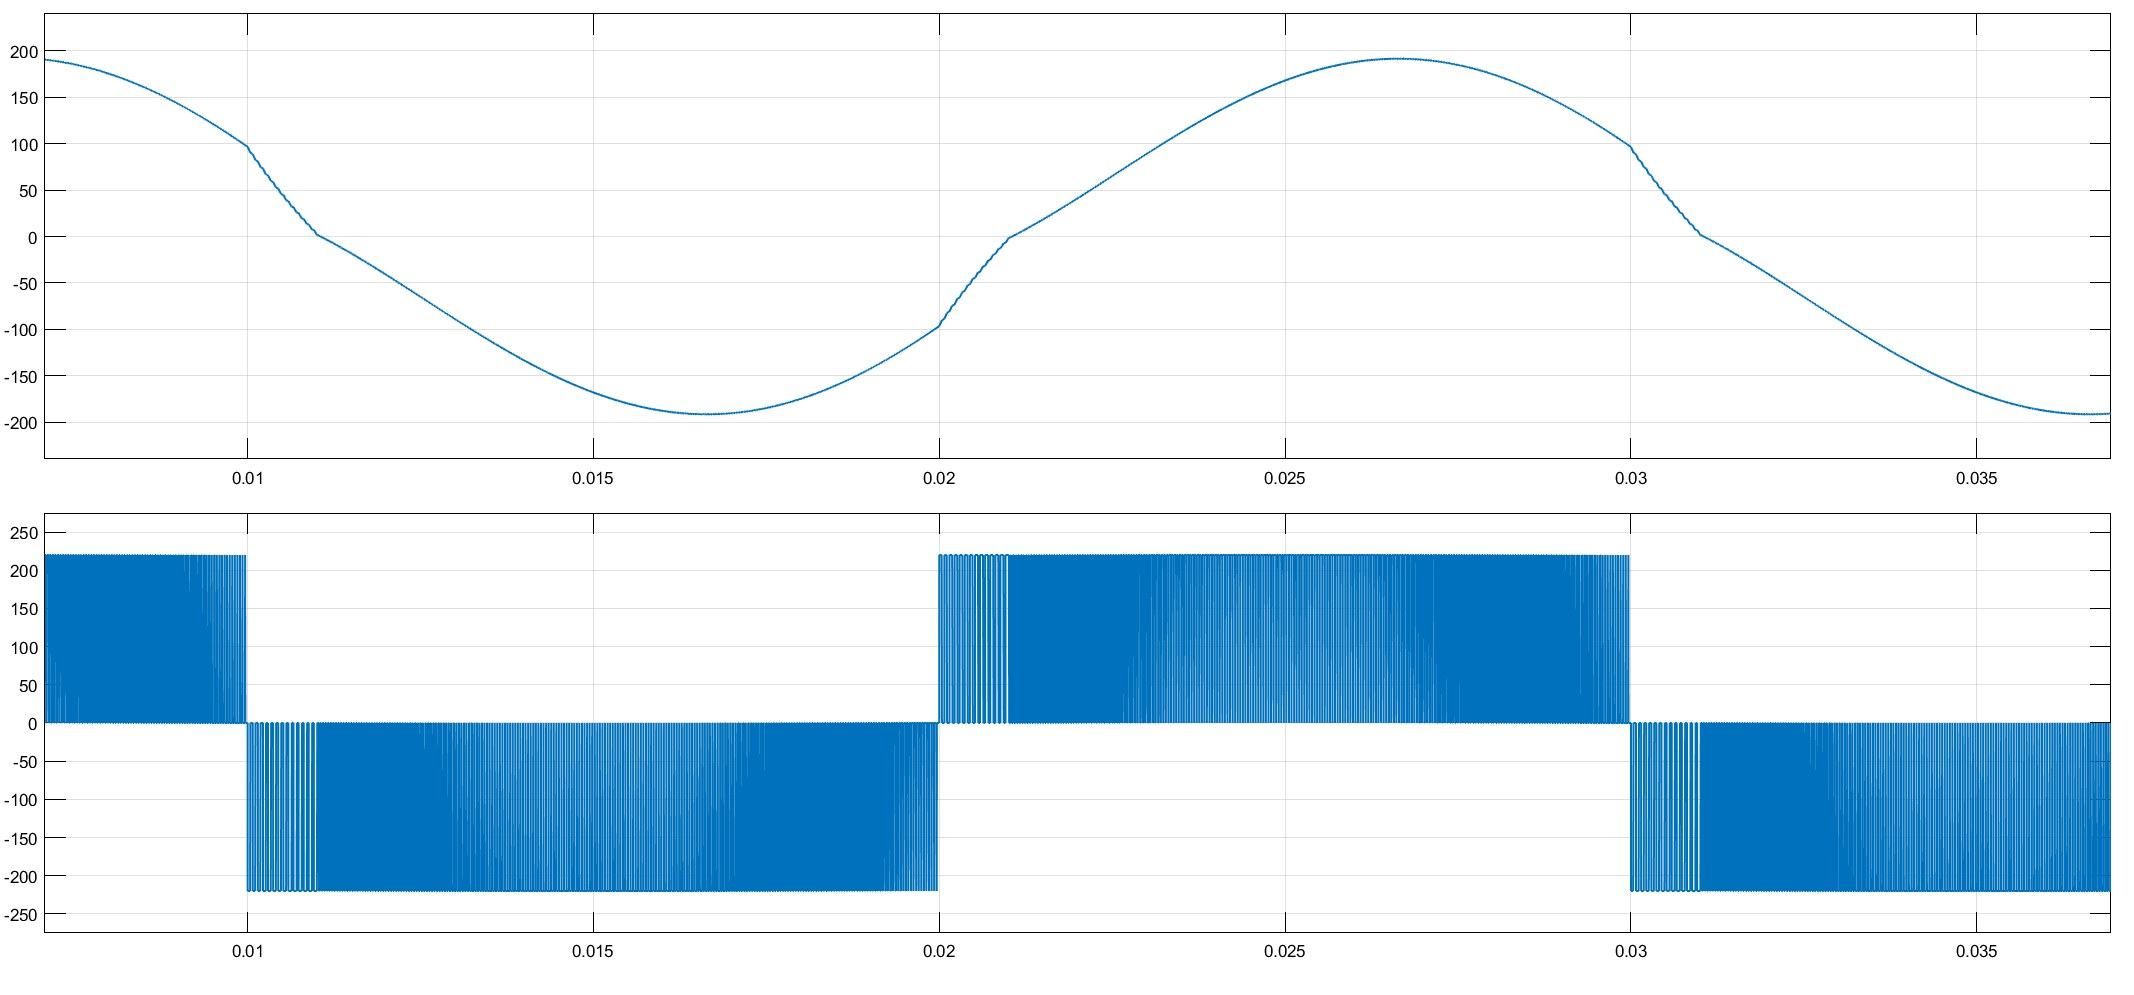
\includegraphics[width=\columnwidth]{figures/wave_heric_bipolar_out.jpg}
\caption{HERIC with bipolar SPWM: (top) filtered and (bottom) unfiltered output voltage. The kinks of the filtered voltage at the zero crossings (0.01~s, 0.02~s, 0.03~s) are the source of the roughly constant 9\% low-order THD.}
\label{fig:outHB}
\end{figure}

\subsection{CM-resonance analysis across cases}
Table~\ref{tab:res} compares the predicted resonance with the leakage peaks observed in the sweeps. The dominant peaks agree with $\fres$ (or $\fres/3$ and $2\fres$ for the H4 bipolar case) to within about 5\%, which is comparable to the sweep resolution of 0.5--1~kHz. The exception is the minor 5-kHz hump of the H4 bipolar case, which lies 14\% below $\fres$, outside the sweep resolution, and is therefore not explained by the first-order model (Section~\ref{sec:limits}). The agreement is not proof that the resonance mechanism is the only cause, but it is strong evidence, since the two values of $\Leq$ differ by a factor of nine and the peaks moved accordingly from about 2~kHz to about 6~kHz.

\begin{table}[!t]
\renewcommand{\arraystretch}{1.2}
\caption{Predicted CM resonance versus observed leakage peaks}
\label{tab:res}
\centering
\footnotesize
\begin{adjustbox}{max width=\columnwidth}
\begin{tabular}{lcccc}
\toprule
Case & Pred.\ $\fres$ (kHz) & Observed peak (kHz) & Relation & Deviation$^{e}$ (\%) \\
\midrule
H4, unipolar   & 1.94 & 2.0 & $\fsw=\fres$ & 3.1 \\
H4, bipolar (major) & 5.81 & 2.0 & $\fsw=\fres/3$ & 3.3 \\
H4, bipolar (major) & 5.81 & 12 & $\fsw=2\fres$ & 3.3 \\
H4, bipolar (minor) & 5.81 & 5 & $\fsw=\fres$ & 14 \\
HERIC, unipolar & 5.81 & 6.0 & $\fsw=\fres$ & 3.3 \\
HERIC, bipolar  & 5.81 & 5.5 & $\fsw=\fres$ & 5.3 \\
\bottomrule
\multicolumn{5}{p{0.95\columnwidth}}{\footnotesize $^{e}$Deviation $=|f_{\mathrm{peak}}-f_{\mathrm{pred}}|/f_{\mathrm{pred}}$, with $f_{\mathrm{pred}}$ the predicted frequency given in the Relation column ($\fres$, $\fres/3$ or $2\fres$), read from the sweep plots; the sweep step is 0.5--1~kHz.}
\end{tabular}
\end{adjustbox}
\end{table}

\emph{Frequency-selection rule.} A practical rule that follows from the results is to keep the switching frequency away from the resonance, from its sub-multiples and, as observed once, from twice its value: $0.8\fres<k\fsw<1.2\fres$ must be avoided for $k=1,2,3$, together with $1.6\fres<\fsw<2.4\fres$, and $\fsw>2.4\fres$ is preferable whenever the efficiency and the switching loss permit. For the H4 bipolar case ($\fres=5.81$~kHz) this excludes about 1.6--2.3~kHz, 2.3--3.5~kHz, 4.6--7~kHz and 9.3--14~kHz, which contain all three leakage peaks of this case (2, 5 and 12~kHz). The rule should be validated for other values of $\Cpv$ (the parasitic capacitance depends on humidity and surface conditions, which shifts $\fres$) and by measurement.

\subsection{Cross-topology comparison}
Table~\ref{tab:summary} summarizes the operating points of the four cases. Within the HERIC pair, which has identical parameters, bipolar SPWM leaks 3.53~mA versus 40.27~mA for unipolar SPWM, a ratio of about 11 at the respective operating points (about 8 at 26~kHz for which both curves are available), but at the cost of a THD of 9.11\% versus 0.05\%.

The H4 and HERIC cases were simulated with different DC voltages, filter inductances and load resistances (Table~\ref{tab:params}), so the estimated output power ranges from about 0.5~kW to 7.4~kW. Consequently, the leakage, efficiency and THD of H4 and HERIC in Table~\ref{tab:summary} should not be used to rank the topologies in absolute terms. For example, the H4 bipolar leakage (14~mA at 40~kHz) and the HERIC bipolar leakage (3.53~mA) differ in $\Vdc$ by a factor of 2.1 and in power by a factor of more than four. Within each case, however, the dependence on the switching frequency is a clean single-factor experiment. A common-parameter re-simulation is needed for a topology ranking and is planned.

\begin{table*}[!t]
\renewcommand{\arraystretch}{1.2}
\caption{Selected operating points and extremes (simulation)}
\label{tab:summary}
\centering
\footnotesize
\setlength{\tabcolsep}{3.5pt}
\begin{adjustbox}{max width=\textwidth}
\begin{tabular}{lcccccc}
\toprule
Case & Point & $I_{\mathrm{leak}}$ & $\eta$ & THD & Worst & Compliant \\
 & (kHz) & (mA) & (\%) & (\%) & peak (mA)$^{a}$ & from (kHz)$^{a}$ \\
\midrule
H4, unipolar & 8.5 & 15.4 & 97.18 & 0.16 & $\approx$750 @ 2 & $\ge 3$ \\
H4, bipolar & 40 & 14 & 97.72 & 0.10 & $\approx$500 @ 2 & see text \\
HERIC, unipolar & 26 & 40.27 & 98.97 & 0.05 & $\approx$4000 @ 6 & $\gtrsim 9$ \\
HERIC, bipolar & 13.5 & 3.53 & n/a & 9.11 & $\approx$15 @ 5.5 & all \\
\bottomrule
\end{tabular}
\end{adjustbox}\\[2pt]
\begin{minipage}{0.97\textwidth}\footnotesize
$^{a}$Read from the sweep figures; ``compliant'' means RMS leakage $<300$~mA. For H4 bipolar the leakage exceeds 300~mA near 2 and 12~kHz.
\end{minipage}
\end{table*}
